%%
%% Beginning of file 'sample.tex'
%%
%% Modified 2005 December 5	
%%
%% This is a sample manuscript marked up using the
%% AASTeX v5.x LaTeX 2e macros.

%% The first piece of markup in an AASTeX v5.x document
%% is the \documentclass command. LaTeX will ignore
%% any data that comes before this command.

%% The command below calls the preprint style
%% which will produce a one-column, single-spaced document.
%% Examples of commands for other substyles follow. Use
%% whichever is most appropriate for your purposes.
%%
%%\documentclass[12pt,preprint]{aastex}
%% manuscript produces a one-column, double-spaced document:

%\documentclass[manuscript]{aastex}
%\documentclass[iop]{emulateapj}
\documentclass[preprint]{emulateapj}
%\documentclass[iop,numberedappendix]{emulateapj}
%\usepackage{url}

%% preprint2 produces a double-column, single-spaced document:

 %\documentclass[preprint2]{aastex}

%% Sometimes a paper's abstract is too long to fit on the
%% title page in preprint2 mode. When that is the case,
%% use the longabstract style option.

 %\documentclass[preprint2,longabstract]{aastex}

%% If you want to create your own macros, you can do so
%% using \newcommand. Your macros should appear before
%% the \begin{document} command.
%%
%% If you are submitting to a journal that translates manuscripts
%% into SGML, you need to follow certain guidelines when preparing
%% your macros. See the AASTeX v5.x Author Guide
%% for information.
\usepackage{color}
\usepackage{cancel,soul,ulem} 

\def\hi{H{\sc i}}
\def\arcsec{\hbox{$^{\prime\prime}$}}
\def\arcmin{\hbox{$^{\prime}$}}
\def\deg{$^\circ$}
\def\cm2{cm$^{-2}$}
\def\cc{cm$^{-3}$}
\def\kms{km s$^{-1}$}
\def\s{s$^{-1}$}
\def\nh3{NH$_3$}
\def\n2h{N$_2$H$^+$}
\def\co{$^{12}$CO}
\def\13co{$^{13}$CO}
\def\c18o{C$^{18}$O}
\def\hc3n{HC$_3$N}
\def\h2{H$_2$}
\def\nh{n(H$_2$)}
\def\cp{C$^+$}
\def\lp{\>\> .}
\def\lc{\>\> ,}
\def\Ms{$M_{\odot}$}
\def\mic{$\mu$m}
\def\Av{A$_V$}
\def\xco{$X_{co}$}

\def\aj{AJ}
\def\aaps{A\&AS}
\def\aap{A\&A}
\def\apjs{ApJS}
\def\nat{Nature}
\def\apj{ApJ}

\newcommand{\chg}[1]{\textbf{\color{green}#1}}
\newcommand{\chb}[1]{\textbf{\color{blue}#1}}
%\newcommand{\st}[1]{\textbf{\color{red}\sout{#1}}}

\newcommand{\rmnum}[1]{\romannumeral #1}
\newcommand{\Rmnum}[1]{\expandafter\@slowromancap\romannumeral #1@}
\makeatother

\shorttitle{Quantifying Dark Gas through OH Absorptions toward Continuum Sources}
\shortauthors{Li et al.}

\begin{document}

\title{Does OH Trace the Dark Molecular Gas (DMG)? }% Force line breaks with \\

\author{Di Li\altaffilmark{1,2}, 
Ningyu Tang\altaffilmark{1,3},
Hiep NGUYEN\altaffilmark{4,5},
J. R. Dawson\altaffilmark{4,5},
Carl Heiles\altaffilmark{6},
Duo Xu\altaffilmark{1,3},
Zhichen Pan\altaffilmark{1,3},
and the PRIMO collaboration
} 

\altaffiltext{1}{National Astronomical Observatories, CAS, Beijing 100012, China; Email: dili@nao.cas.cn, nytang@nao.cas.cn}
\altaffiltext{2}{Key Laboratory of Radio Astronomy, Chinese Academy of Science}
\altaffiltext{3}{University of Chinese Academy of Sciences, Beijing 100049, China}
\altaffiltext{4}{Department of Physics and Astronomy and MQ Research Centre in Astronomy, Astrophysics and Astrophotonics, Macquarie 
 University, NSW 2109, Australia}
\altaffiltext{5}{Australia Telescope National Facility, CSIRO Astronomy and Space Science, PO Box 76, Epping, NSW 1710, Australia}
\altaffiltext{6}{Department of Astronomy, University of California, Berkeley, 601 Campbell Hall 3411, Berkeley, CA 94720-3411}

\begin{abstract}
%A growing body of evidence has been supporting the existence of so-called ``dark molecular gas" (DMG), which is invisible in the most common tracer of molecular gas, i.e., CO rotational emission. DMG is believed to be the main gas component of the 
%intermediate extinction region between A$\rm_V$$\sim$0.05--2 mag, roughly corresponding to the self-shielding threshold of \h2\ and \13co. 
%To quantify DMG relative to \hi\ and CO, we are pursuing three observational techniques, namely, \hi\ self-absorption, OH absorption, and %TeraHz \cp\ emission. In this paper, we focus on preliminary results from a CO and OH absorption survey of DMG candidates.
%Our analysis show that the OH excitation temperature is close to that of the Galactic continuum background and that OH is a good DMG tracer  co-existing with  molecular hydrogen in regions without CO. Through systematic ``absorption mapping" by Square Kilometer Array (SKA) and ALMA, we will have unprecedented, comprehensive knowledge of the ISM components including DMG in terms of their temperature and density, which will impact our understanding of galaxy evolution and star formation profoundly.

Hydroxyl (OH) is supposed to be abundant in diffuse interstellar molecular gas as it forms along with \h2\ under similar conditions and within similar extinction range. Despite being the first interstellar molecule detected in radio bands, systematic mapping of OH remains rare. We analyzed absorption measurements of the $\Lambda$-doubling transitions of OH at 1665 MHz and 1667 MHz toward 43 continuum sources, along with the J=1-0 emission of CO, \13co and \c18o, and the J=3-2 of CO. The OH data were taken during the  Millennium survey and were unpublished until now. The 3mm data were taken with the 13.7m Delingha telescope in Qinghai, China and the 1mm data with the 10.4m dish of the  Caltech Submillimeter Observatory (CSO). The excitation temperatures of OH were found to be generally close to those of the background ($\sim$3-4K), providing a plausible explanation for the difficulty of detecting such an abundant molecule in emission. The detection rate of OH in the intermediate extinction rage (\Av\ $\sim$ 0.05--2 mag) is approximately constant, while that of CO seems to grow with extinction. We conclude that OH is abundant in diffuse molecular gas and OH absorption a good tracer of DMG due to its low excitation. The self-shielding threshold of CO formation is not apparent in our data, supporting the existence of widely distributed diffuse CO gas. The upcoming highly sensitive radio telescopes, namely, FAST and SKA, will make feasible systematic inventory of diffuse molecular gas through decomposing cm molecular  (e.g.\ OH and CH) absorption profiles toward background continuum sources with numbers orders of magnitude higher than those available now.



 %With ON-OFF observations, we derive excitation temperature and optical depth of decompose 48 OH components. Optical depth of  OH main lines are  less than 0.22 for all components. Most OH components are in non local thermal equilibrium (LTE), making deviation between excitation temperature of 1665 and 1667 MHz lines. The difference of excitation temperature of 1665 and 1667 MHz lines, $|T_{ex}(1667)-T_{ex}(1665)|$ is less than 2 K. No correlation between \hi\ and OH was found.  Compared to CO follow up observations, 3 components have OH absorption but are absent in CO. They are called as ``CO dark molecular gas".  \hi\ column density range of DMG clouds are smaller than that of molecular and cold \hi\  gas, indicating that DMG take a small portion in the evolution stage of interstellar medium. systematic ``absorption mapping" by Square Kilometer Array (SKA) and ALMA, we will have unprecedented, comprehensive knowledge of the ISM components including DMG in terms of their temperature and density, which will impact our understanding of galaxy evolution and star formation profoundly. 

\end{abstract}

\keywords{ISM: clouds --- ISM: evolution --- ISM: molecules.}

\section{Introduction}
 The two relatively denser phases of the interstellar medium (ISM) are the atomic Cold Neutral Medium (CNM) traced by the \hi\ $\lambda$21cm hyperfine structure line and the `standard' molecular (H$_2$) clouds , usually traced by CO. CO is the most important tracer of molecular hydrogen, which remains largely invisible due to its lack of emission in the temperature range of molecular ISM. Empirically, CO intensities have been used as an indicator of the total molecular mass in the Milkyway and in galaxies through the so-called ``X-factor" (\xco) with numerous  caveats.  Gases in these two phases dominate the masses of star forming clouds on a galactic scale. The measured ISM gas mass from \hi\ and CO is the foundation of many key quantities in understanding galaxy evolution and star formation, such as the star formation efficiency.
 
 A growing body of evidence, however,  indicates the existence of gas traced by neither \hi\ nor CO.  Comparative studies (e.g.\ de Vries et al.\ 1987) of Infrared Astronomy Satellite (IRAS) dust images and gas maps in \hi\ and CO revealed apparent `excess' of dust emission. The Planck collaboration (2011) clearly show excess dust opacity  in the intermediate extinction range $A_V \sim$ 0.05--2 mag, roughly corresponding to the self-shielding threshold of \h2\ and \13co, respectively. The missing gas, or rather, the undetected gas component is widely referred to as dark gas, popularized as a common term by Grenier et al.\ (2005), who found more diffuse gamma-ray emission observed by Energetic Gamma Ray Experiment Telescope (EGRET) than what can be explained by cosmic-ray interacting with the H-nuclei, the total quantity of which were presumed to be [N(\hi)+\xco*CO]. Observation of the TeraHz fine structure \cp\ line also help reveal dark gas in that the \cp\ line strength in diffuse gas is stronger than what can be produced by collisional excitation with only \hi\ gas (Langer et al.\ 2010; Pineda et al.\ 2013). A minority of the ISM communities argued that dark gas can be explained by underestimated HI opacities (Fukui et al.\ 2014), which is in contrast with some other recent works (Stanimirovi{\'c} et al.\ 2014).  We focus here on the dark molecular gas (DMG), or more specifically CO-dark molecular gas.
% \begin{figure}
%\includegraphics[width=0.95\linewidth]{fig/aa16479-11-fig6.pdf}
%\caption{This figure is adopted from the Figure 6 in Planck (2011). Correlation plots between the gas column density as traced by [HI+X$_{CO}$*CO] and dust optical depth at IRAS 100 \mic\ (upper left), HFI 857 GHz (upper right), 545 GHz (lower left) and 353 GHz (lower right). The color scale represents the density of sky pixels on a log scale. The blue dots show a binned average representation of the correlation. The red line shows the best linear correlation derived at low values. The vertical lines show the positions corresponding to A$\rm_V$ = 0.37 mag and A$\rm_V$ = 2.5 mag.  A single CO X-factor X$_{CO}$ = 2.3 $\times10^{20}$ \h2\ cm$^{-2}$/(K km \s) was used. }
%\label{fig1}
%\end{figure}

ISM chemistry and PDR models predict the existence of \h2\ in regions where CO is not detectable (Wolfire et al.\ 2010).
 CO can be of  low abundance due to photo-dissociation  in unshielded regions and/or can be heavily sub-thermal due to lack of collision in diffuse gas.  OH, or Hydroxyl, is the first interstellar molecule detected in radio bands (Weinreb et al.\ 1963). It can form quickly through a series of charge exchange reactions ({\em this may not be the right terminology? Does anybody know what these reactions are called})  initiated by cosmic ray once \h2\ becomes available (van Dishoeck \& Black 1988). 
 \begin{equation}
\mathrm{OH+C^+\to CO^++ H}\label{eq1} \lc
\end{equation}
\begin{equation}
\mathrm{CO^++H_2 \to HCO^++ H}\label{eq2} \lc
\end{equation}
\begin{equation}
\mathrm{HCO^++e^-\to CO+ H}\label{eq3}  \lp
\end{equation}
%OH can also form on grains (??? tny: yes, but that contributes little to OH formation.). 
Wide-spread and abundant OH along with HCO$^+$ and \cp\ are expected. It is thus puzzling why large scale OH surveys of ISM has been so rare  in the half century following its discovery.  The emission strength of OH is weak except for relatively compact and dense molecular clouds (Allen et al.\ 2015) in the Milkyway.  More than a thousand hours of Arecibo time were spent on searches for OH in other galaxies with mostly negative results (e.g.\ Schmelz \& Baan 1988). 
In contrast, Dickey et al.\ (1981) found OH in absorption against high Galactic latitude continuum sources. Extensive  absorption measurements by Liszt \& Lucas (1996) and Lucas \& Liszt(1996) found that OH and HCO$^{+}$ are commonly observed against such sources and have a tight correlation between each other. Lucas \& Liszt(1996) found that $\thicksim$30\% of continuum sources having \hi\ absorption exhibit HCO$^{+}$ absorption. In light of these results, the dearth of OH emission should be attributed to the excitation condition of OH rather than its abundance.
 
 %The observed antenna temperature $T_A=(T_{ex}-T_{C})(1-e^{-\tau})$, where $T_C \sim 3.5$ K is the continuum background temperature at L-band, comprising of the CMB and the galactic synchrotron emission.  When $T_{ex}$ approaches $T_C$, the apparent signal from certain line emission vanishes. Such gas, however, is suitable for absorption study when the telescope is trained toward background sources with $T_C \gg T_{ex}$ as is the case when observing quasars and/or HII regions.

Heiles \& Troland (2003) published the  Millennium survey of 21-cm line absorption toward 79 continuum sources. The ON-OFF technique and Gaussian decomposition analysis allowed them to provide direct measurements of the excitation temperature and density of \hi\ components spreading throughout the Milkyway. The large gain of Arecibo and the substantial integration time spent on each source make the Millennium survey one of the most sensitivity survey of the diffuse ISM gas components.
Among the significant findings is the fact that a substantial fraction of the CNM lies below the canonical 100K temperature predicted by phased ISM models (Field, Goldsmith \& Habing 1969; McKee \& Ostriker 1977) for maintaining pressure balance. The L-wide receiver at Arecibo allows for simultaneously observation of \hi\ and OH, which was accomplished by the Millennium survey. The OH absorption data were not published yet. We conducted  3mm and 1mm CO observations toward the Millennium sources. We carried out a combined  of OH and CO in terms of their excitation, abundances, implications for conditions of the DMG.

This paper is organized as follows: In section \ref{sec:observations}, we describe the observations of \hi, OH, and CO. In section \ref{sec:oh_properties}, we analyse the OH properties. In section \ref{sec:comparison}, we show study the relation between these three spectral tracers. Discussions and conclusions are presented in section \ref{sec:abs_survey} and section \ref{sec:conclusion}, respectively. 

%\begin{figure}
%\includegraphics[width=0.96\linewidth]{fig/pdr_new.eps}
%\caption{A schematic view of photo-dissociation region (Tielens  2005). It shows the locations of different transition layers. We add the blue pane to indicate the possible location of OH.}
%\label{pdrmodel}
%\end{figure}

% \section{A Multi-transition CO Survey of Millennium Sources}
\section{Observations}
\label{sec:observations}

\subsection{\hi\ and OH}
\label{subsec:oh}
Heiles \& Troland (2001; 2003a, b) developed and implemented the so-called  Z17 method for obtaining and analyzing absorption spectra toward continuum sources. Such method required half of the integrations spent on source with the remaining time divided evenly among 16 OFF positions. The OFF  spectra were then used to reconstruct the background gas spectrum, were there no continuum source. 
During the Millennium survey, the $\Lambda$-doubling transitions of OH at1665 and 1667 MHz  were obtained simultaneously with those of \hi\ with the Arecibo L-wide receiver. 
The bandwidth of OH observation was 0.78 MHz. The channel width of the observation was 381 KHz, corresponding to a velocity resolution of 0.068 \kms. A RMS of ???mK per channel was achieved with ??? hours of total integration time. Forty-nine out of 77 Millennium sightlines exhibited OH absorption. The distribution of these sources in the galactic coordinate is presented in Fig.~\ref{fig:posdistri}. 
\begin{figure}
\includegraphics[width=1.0\linewidth]{fig/detection.eps}
\caption{The location of sources in galactic coordinate. Open circle represents the source with \hi\ absorption. Square represents the source with absorption component in OH.  Red dot represents the source with CO transition components, and these CO components correspond to all the absorption components in OH. Blue dot represents the source with CO transition components, and these CO components correspond to some of the absorption components in OH, but there are no detectable CO transition corresponding to the rest of absorption components in OH. We call these kind of sources ``part CO detection".  }
\label{fig:posdistri} 
\end{figure}

\subsection{CO}
\label{subsec:CO}
	We conducted a follow-up CO survey of all 48 Millennium sight-lines with OH absorption.  The J=1-0 transitions of CO, \13co, and \c18o\ were observed with the Purple Mountain Observatory Delingha (PMODLH) 13.7 m telescope, Chinese Academy of Sciences. The data of these three transitions were taken simultaneously  with the 3mm SIS receiver in March 2013, May 2013, May 2014, and May 2016. FFTS wide-band spectral backend has a bandwidth of 1 GHz at a frequency resolution of 61.0 kHz, which corresponds to 0.159 \kms at 115.0 GHz and  0.166 \kms at 110.0 GHz. Position-switch mode was  used with reference positions selected from IRAS Sky Survey Atlas\footnote{$http://irsa.ipac.caltech.edu/data/ISSA/$}.  The system temperature varied from 210 K to 350 K for CO, and 140 K  to 225 K for  \13co and \c18o bands. The resulting RMS is $\sim$ 60 mK for a 0.159 \kms\  channel for $^{12}$CO and $\sim$ 30 mK for a 0.166 \kms\  channel for $^{13}$CO and C$^{18}$O. respectively.    
	% FFTS1 of CSO backend 
	
	The \co\  J=2-1 data for 45 sources and J=3-2 data for 8 sources with strong CO emission were taken with the  Caltech Submillimeter Observatory (CSO) 10.4m on top of Mauna Kea in July, October, and December of 2013.  The system temperature varied from 230 to 300 K for CO(2-1), resulting a rms of $\sim 35$ mK at velocity resolution of 0.16 \kms of FFTS1W spectrometer.   $^{12}$CO(J=3-2) observations of  6 sources were observed with FFTS1W spectrometer at velocity resolution of 0.11 \kms, deriving a spectral rms of $\sim$ 0.2 K.  $^{12}$CO(J=3-2) observations of  2 sources, 3C154 and T0629+10, were observed  with AOS5 spectrometer at velocity resoluiton of  0.56 \kms. The rms values are 0.38 K and 0.14 K for 3C154 and T0629+10, respectively.
		% 0.56  3C154  T0629+10
	%(??? due to a problem of spectroscopy??? what problem? Why don't we just smooth everything to 0.56 \kms?).  ??? Please describe the integration time, RMS, etc. here. 
	
	Three sightlines of the $^{12}$CO J=2-1 line were observed with IRAM telescope through frequency switch mode in May 22 to May 23, 2016.  Depending on different system temperatures, the observation time varied from  30 min to 90 min to reach a rms that is less than 20 mK at a velocity resolution of 0.25 \kms.
	
	The astronomical software package Gildas/CLASS\footnote{$http://www.iram.fr/IRAMFR/GILDAS/$} was used for baseline removing, spectra combining and gaussian fitting of CO data. 

\section{OH Properties}
\label{sec:oh_properties}

\subsection{Detecting OH in Absorption and Emission}
\label{sec:oh_emi_abs}

Our primary detection scheme was OH in absorption against the background continuum sources used in the Millennium survey. These sources typically had S $\gtrsim 2$ Jy, so produced antenna temperatures in excess of about 20 K at Arecibo. We decomposed all OH lines into Gaussian components and made the histogram of the peak optical depth for each component (Figure \ref{fig:taupeak_hist}). 

The OH lines are much stronger in absorption than in emission. This is easy to understand when considering the excitation temperature. For a frequency-switched emission spectrum of a single OH feature having peak optical depth $\tau$ seen against a continuum background brightness temperature $T\rm_C$, the observed antenna temperature $T\rm_A$ is 
 \begin{equation}
T_A=(T_{x}-T_{C})(1-e^{-\tau}),
\label{eq4} 
\end{equation}
where  $T\rm_x$ is the OH line excitation temperature, $T\rm_C$ includes the Cosmic Background Radiation (CBR) and  the Galactic synchrotron background, which we obtained from  408 MHz map (Haslam et al. 1982) and scaled in frequency with spectral index of 2.8. The  background continuum contribution from Galactic HII region may be ignored as the continuum sources we observed are in high Galactic latitude or anti-center longitude.  Owing to our OH line measurements in both absorption and emission, we derive $T\rm_x$. Figure \ref{fig:Tex_hist} shows the histogram of $T\rm_x$ and $T\rm_C$. $T\rm_C$ is typically about 3.5 K, while the range of $T\rm_x$ is from 2 to 15 K - but they peak at low temperatures. Since $T\rm{_A} \propto (T\rm{_x}-T\rm{_C})$, the emission line intensities are significantly reduced. 

As shown in Figure \ref{fig:Tant_hist}, the histogram of antenna temperature rise toward low values, implying sensitivity limited. The peak of low temperature is at about 20 mK, and we expect more lines to be even weaker. This result conforms our conclusion that OH is hard to be detected in emission but much easier to be detected in absorption. 

\begin{figure}
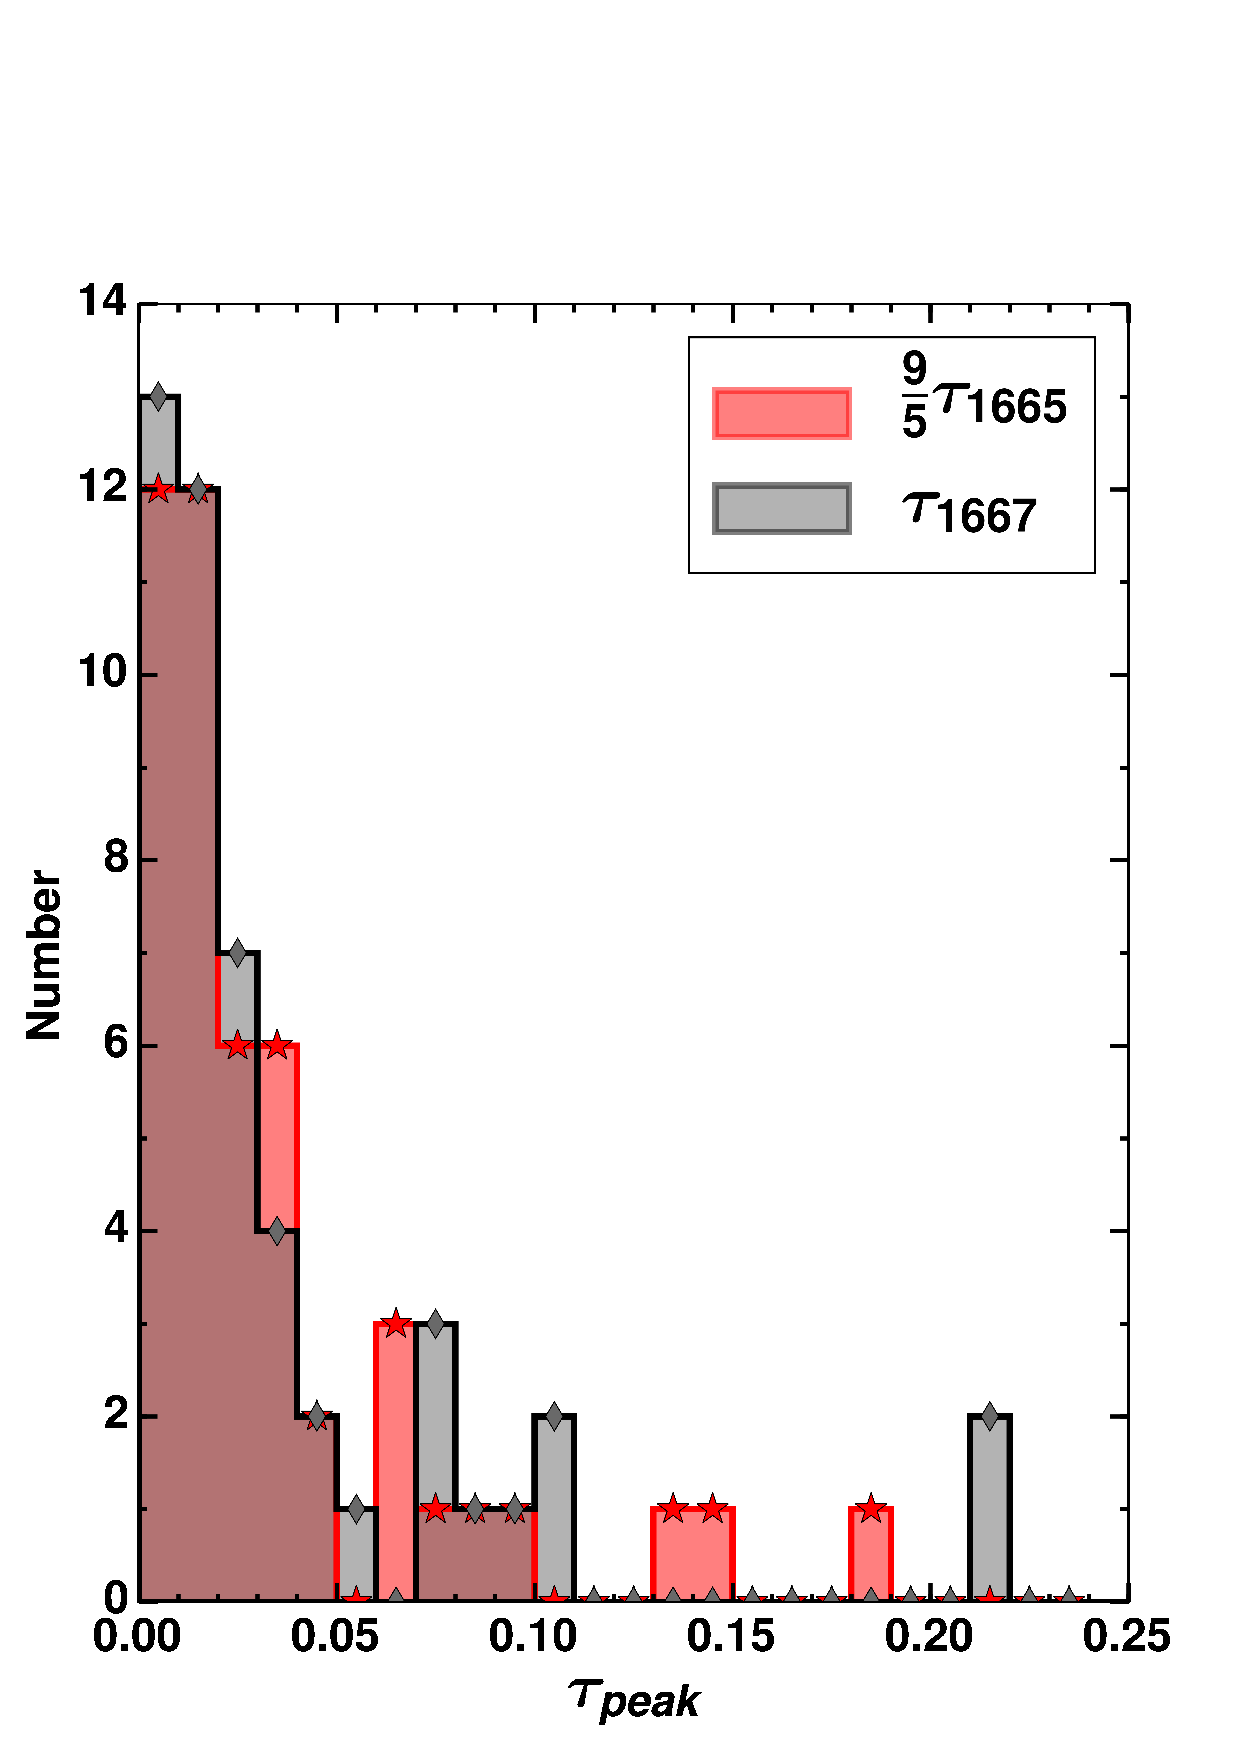
\includegraphics[width=1.0\linewidth]{fig/tau_peak_hist.png}
\caption{Histogram of peak optical depth for the Gaussian components. Black shows OH 1667 MHz and red shows 9/5 times the peak optical depth for OH 1665 MHz line. }
\label{fig:taupeak_hist} 
\end{figure}

\begin{figure}
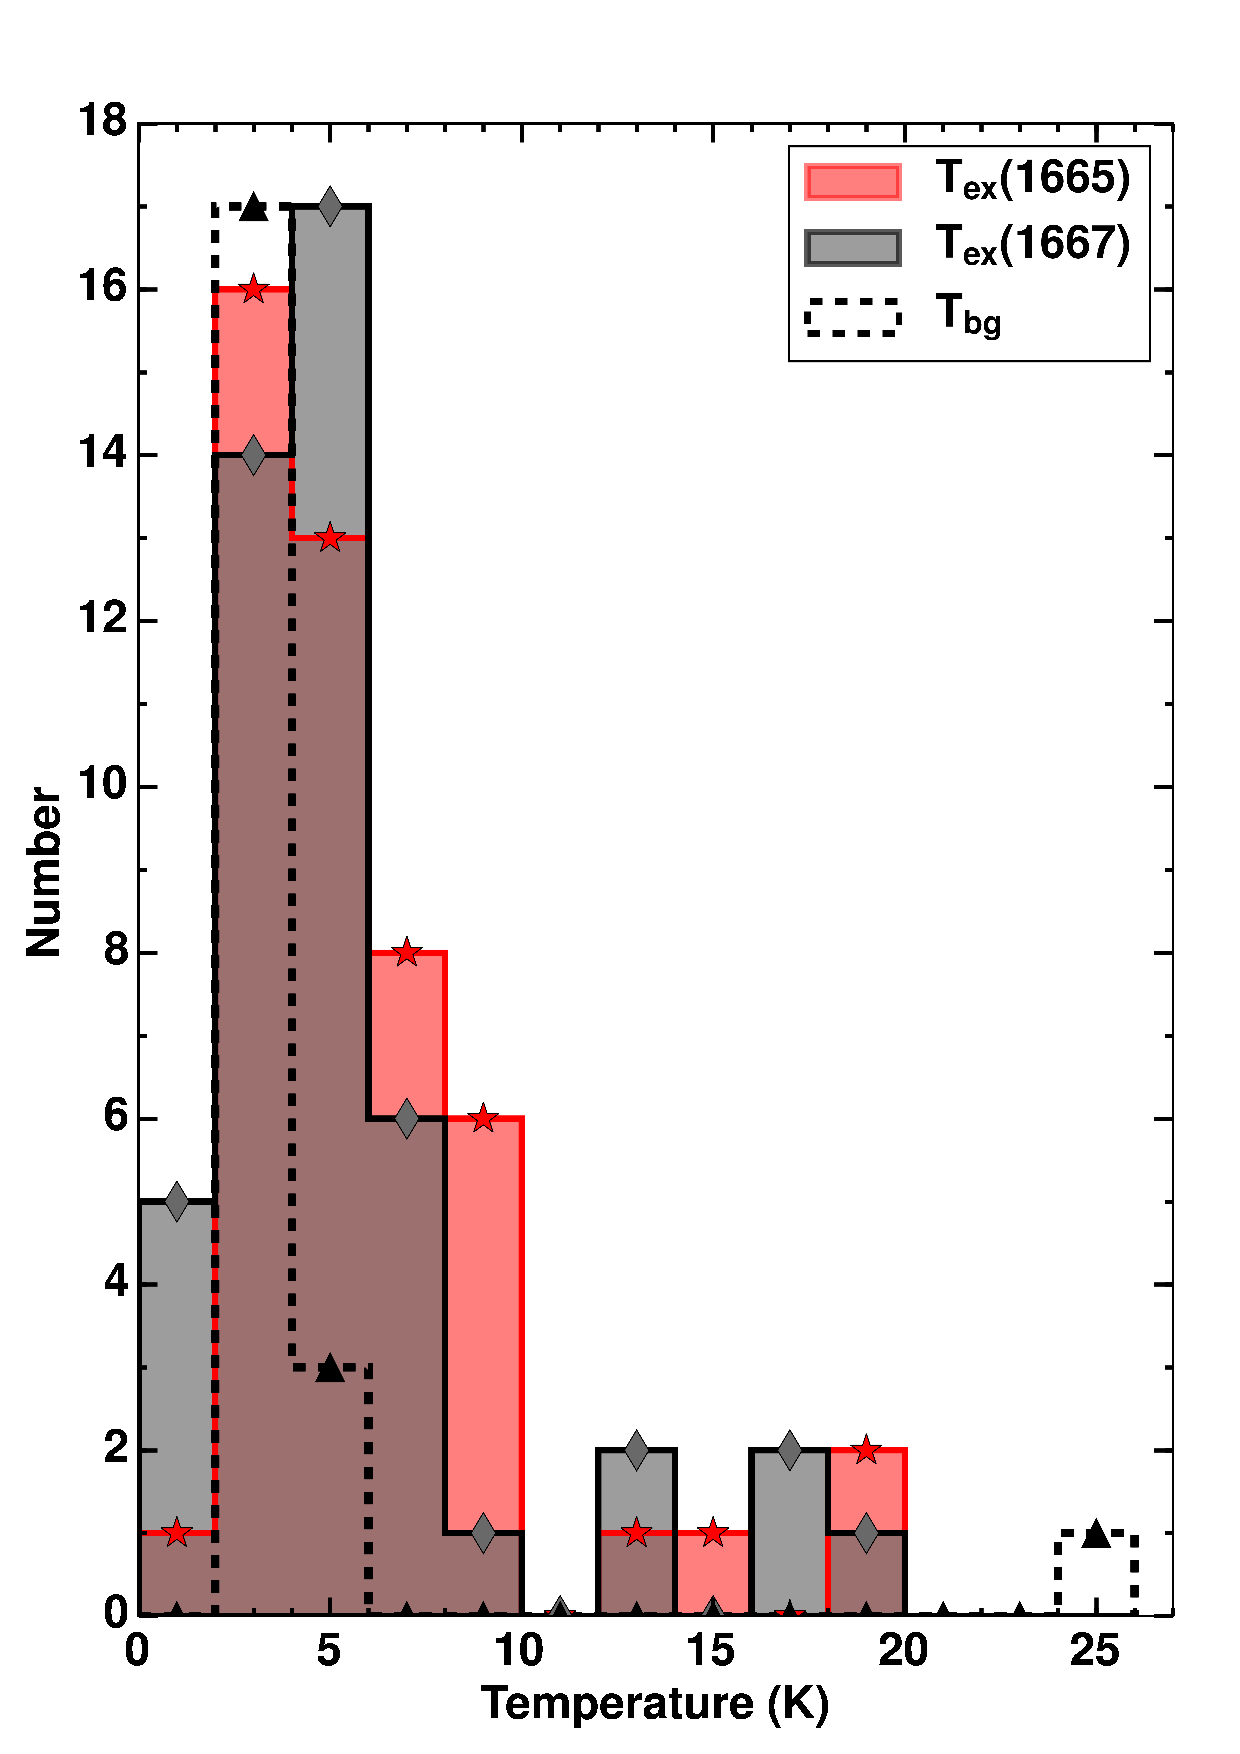
\includegraphics[width=1.0\linewidth]{fig/Tex_hist.png}
\caption{Histogramss of excitation temperature $T\rm_{x}$ for two OH main lines and background continuum temperature $T\rm_C$.}
\label{fig:Tex_hist} 
\end{figure}

\begin{figure}
\includegraphics[width=1.0\linewidth]{fig/Tant_hist.png}
\caption{Histogramss of  antenna temperature for the OH components in emission.}
\label{fig:Tant_hist} 
\end{figure}

\subsection{OH Excitation}
\label{subsec:oh_excitation}

When OH is excited in  local  thermal equilibrium (LTE), the excitation temperature of 1665 and 1667 MHz lines are equal. Under LTE condition, the optical depth ratio between 1667 and 1665 MHz lines is 1.8.  As shown in Figure \ref{fig:delspin_vs_tauratio}, most OH clouds are in non-LTE excitation. The values between excitation temperature of 1667 and 1665 MHz lines, $\Delta T\rm_{ex}$, concentrate in the range of  $|\Delta T\rm_{ex}| < 2$ K.  This is consistent with the value, $|\Delta T\rm_{ex}| \sim 1-2 $ K, derived in previous absorption toward continuum sources (e.g., Nguyen-Q-Rieu et al.\ 1976; Crutcher 1977, 1979; Dickey et al.\ 1981).

In Figure \ref{fig:delspin_vs_tauratio}, there is no evidence that $R_{67/65}$  approaches 1.8 when $|\Delta T\rm_{ex}|$ approaches 0. This may indicate non-thermal excitation of OH gas. 

\begin{figure}
\includegraphics[width=1.0\linewidth]{fig/delspin_vs_tauratio.eps}
\caption{Optical depth ratio ($\tau_{1667}/\tau_{1665}$) as a function of  excitation temperature differences ($T\rm_{ex}(1667)-T_{ex}(1665)$) for 1667 and 1665 MHz lines. The horizontal dotted lines represents 1.8, which is the value when OH is in LTE. Vertical shad region represents  $|\Delta T\rm_{ex}| < 2$ K .}
\label{fig:delspin_vs_tauratio} 
\end{figure}

\section{Comparison betwen Spectral Lines}
\label{sec:comparison}
\subsection{OH and \hi\ }
\label{subsec:hioh}
To check if OH would increase with the column density of \hi, we plot OH column densities derived from the emission/absorption data versus \hi\ column densities, both on a Gaussian component-by-component basis. It requires associating OH components with \hi\ components. This is not so easy. \hi\ components are always wider than OH ones, and the central velocities never line up. Usually there are several OH components for each \hi\ component. The OH column densities in Figure \ref{fig:Noh_vs_NHI} are the sum of of all OH components associated with a single \hi\ component. 

The row of red points at ``zero" on the vertical axis shows that there are a lot of \hi\ components without OH. N(OH) does not increase monotonically with N(\hi). However, this needs further check - to what extent are the \hi\ components break down into small subcomponents.  


\begin{figure}
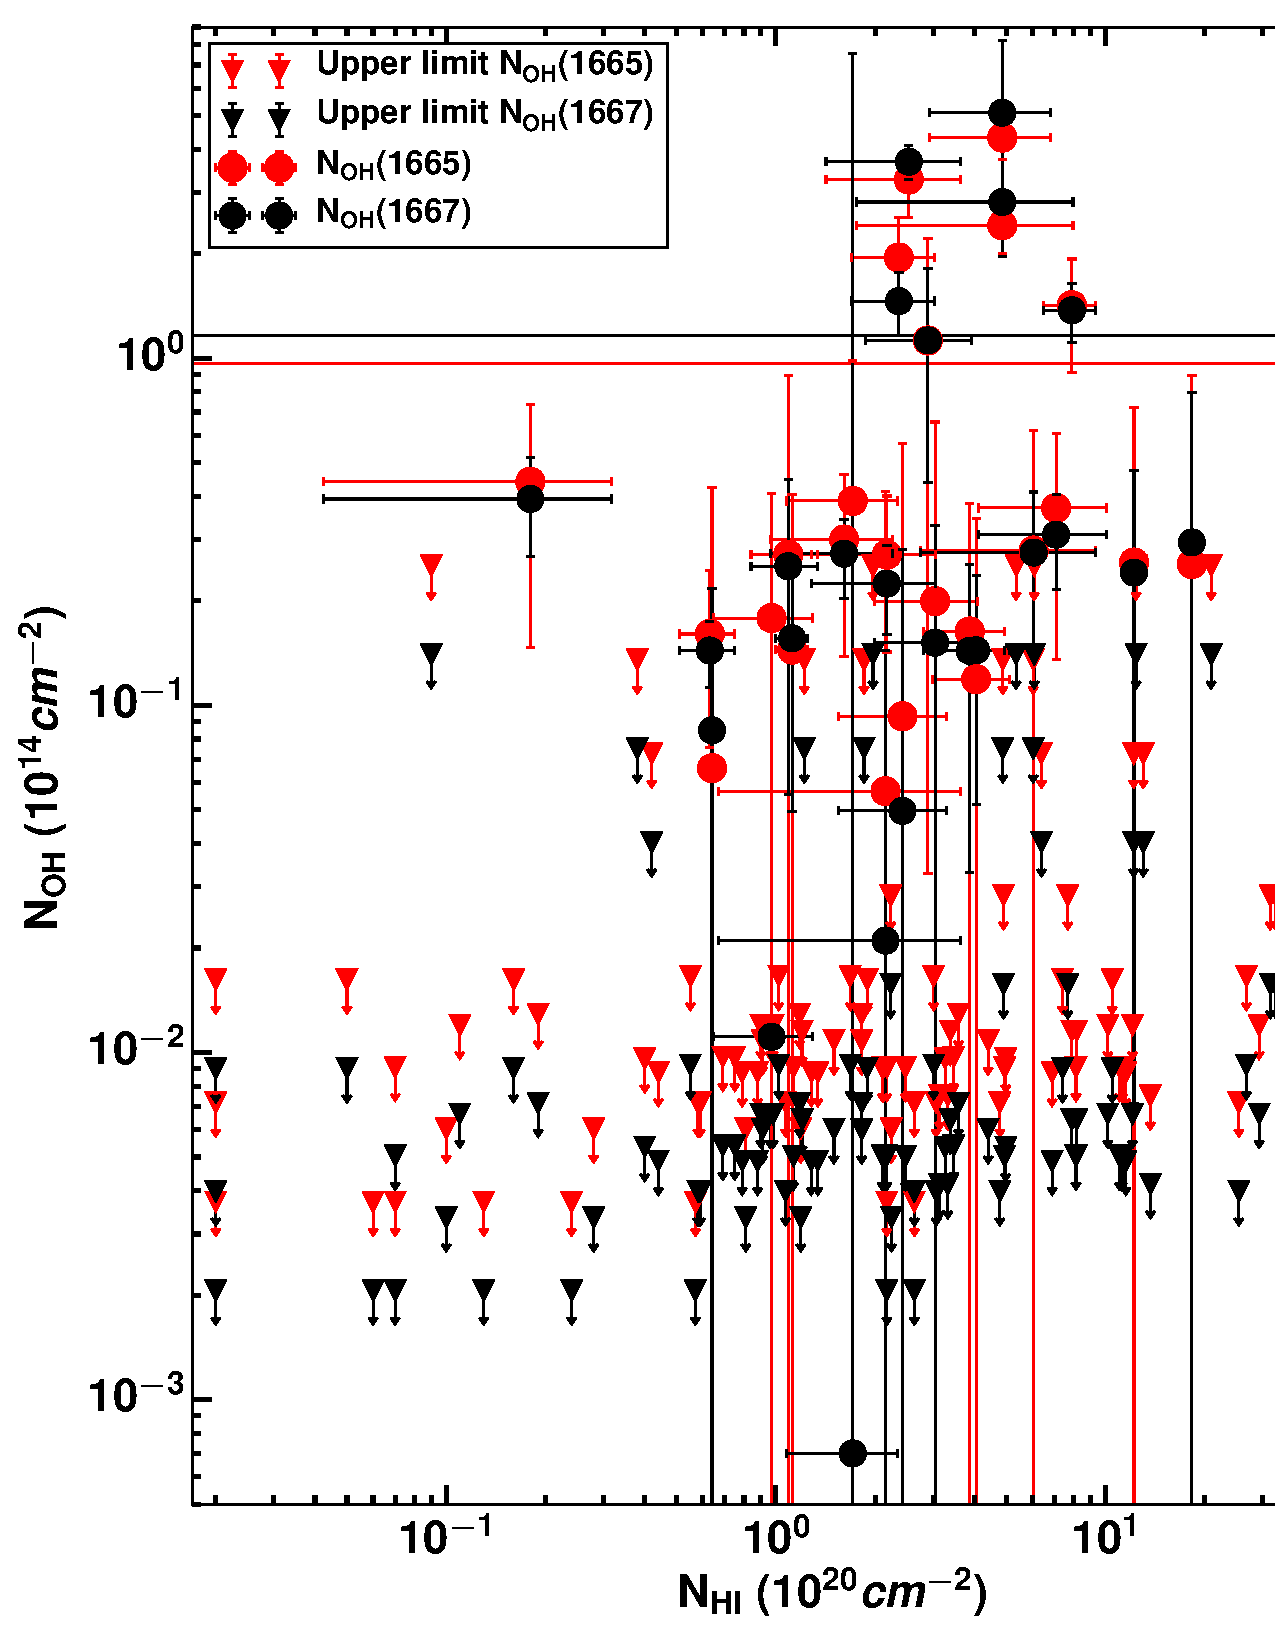
\includegraphics[width=1.0\linewidth]{fig/Noh_vs_NHI.png}
\caption{Histogramss of  antenna temperature for the OH components in emission.}
\label{fig:Noh_vs_NHI} 
\end{figure}

\subsection{OH and CO}
\label{subsec:ohco}

To be added....

\subsection{CO-Dark Molecular Gas}
\label{subsec:darkgas}

We compare the Gaussian components seen in \hi\ absorption, OH absorption, and CO emission.
A total of 115 Gaussian components were detected as specified in Heiles \& Troland (2003). 
Forty-eight such gas components have OH absorption. The majority of these components  have corresponding CO emission, except for 11 components, which are DMG candidates. We have detected 3 components with only CO emission and no OH absorption.
Three representative sets of spectra are shown in Fig.~\ref{fig4}.  Toward 3C192, only \hi\ is present, typical of CNM. 
Toward 3C133, there is a  component with \hi, OH, and several CO and CO isotopologue transitions, which should be 
representative of `normal' molecular clouds. Toward 3C132, there exists a component with \hi\ and OH absorption, but no CO emission in any transition observed. We posit that this is typical of DMG.  The percentage of these three categories are 86\% CNM,  11\% molecular clouds, and 2.4\% DMG.

\begin{figure}[htp]
\includegraphics[width=1.0\linewidth]{fig/spec3.eps}
\caption{Representative spectra. 3C192 sightline has only \hi\ seen in absorption. One component of 3C133 sightline has OH and \hi\ in absorption and CO and its isotopologues in emission. 3C132 sightline has one gas component with both OH and \hi\ , but no detectable CO transitions.}
\label{fig4}
\end{figure}

The column densities of  OH components were calculated as
\begin{equation}
N_{OH}=\frac{8\pi kT_{ex}{{\nu}^2_{1667}}}{A_{1667}c^{3}h}\frac{16}{5}\int \tau_{1667} \,dv \lc
\label{eq5}
\end{equation}
where $A_{1667}=7.778\times 10^{-11} s^{-1}$ is the A-coefficient  and $T_{ex}$ is its excitation temperature calculated based on a
recipe similar to that for \hi\ absorption components in Heiles \& Troland (2003). 

The CO column densities were calculated in two categories. If only the J=1-0 transition of \co\ is detected, the optical depth is assumed to be small and the excitation temperature is assumed to be the same as that of OH. If both \co\ and \13co\ are detected, we derive the optical depth and the excitation temperature based on multiple transitions and Local Thermodynamic Equilibrium (LTE) assumptions. The recipe for deriving CO column densities can be found in Li (2002).

The statistics of \hi\ column density are present in Figure \ref{fig:hist_hi_dg_mo}.  There is an apparent gas column density threshold for OH detection at around A$\rm_V$$\sim$0.05 mag, above which OH and CO have similar distribution.
OH turns out be a good tracer of diffuse gas with `intermediate' extinction, namely, between the self-shielding threshold for \h2\ and \13co.
\begin{figure}
\includegraphics[width=1.0\linewidth]{fig/hist_hi_dg_mo.eps}
\caption{The histogram of \hi\ colunm density for the cold neutron medium(the blue filled rectangle), molecular gas(the green line filled rectangle) and dark gas(the red line filled rectangle).  }
\label{fig:hist_hi_dg_mo}
\end{figure}

\section{Implication of Absorption Survey}
\label{sec:abs_survey}

The expected location, abundance, and optical depth of OH should make it 
an excellent tracer of DMG. Due to insufficient collision in diffuse gas, however, OH is hard to
detect in emission. This is likely the main reason why a galactic scale or even any large-scale OH map has not 
been accomplished. To realize its potential in quantifying dark gas throughout the ISM, the upcoming radio telescopes 
will be needed to conduct comprehensive absorption surveys. The Five-hundred-meter Aperture Spherical radio Telescope (FAST)
started observation in September, 2016. The unprecedented sensitivity of FAST and its early science instruments (Li et al.\ 2013) 
should make feasible a \hi+OH absorption survey, in the mode of the Millennium survey, but with 10 times more sources. Figure \ref{fig:fast_survey} shows distribution of  potential continuum sources those are available to FAST.  The SKA1 will have the survey speed and sensitivity to measure gas absorption with a source density between a few to a few tens per square degree (McClure-Griffiths et al.\ 2014), which means that an all sky ``absorption-image" is feasible and we will have ISM temperature and density  everywhere! Based on similar excitation  and sensitivity considerations,  ALMA is a powerful instrument to obtain systematic and sensitive absorption measurements of millimeter lines in diffuse gas. CO and HCO$^+$ in diffuse gas, in particular, will be much better constrained in terms of excitation temperature and column densities through ALMA absorption observation than emission measurements. Combining both radio and millimeter absorption surveys in the coming decade, we will quantify DMG and provide definitive answers to questions like the global star formation efficiency. 

\begin{figure}
\includegraphics[width=1.0\linewidth]{fig/lab_intg_car.png}
\caption{Distribution of 1773 point continuum sources (blue dots) that are in FAST sky coverage, which is declination range of (-14, 66) degree.  These sources have peak intensity that is greater than 0.75 Jy/beam in NVSS survey. In front observation periods, FAST will adopt drift scan mode. The criterial of 0.75 Jy/beam corresponds 3$\sigma$ detection in absorption for \hi\ gas with optical depth of 0.05 in a drift scan of 10s.  The grey background is integrated \hi\ intensity map from LAB \hi\ survey (Hartmann \& Burton 1997; Arnal et al.\ 2000; Bajaja et al.\ 2005). The coverage of FAST and Arecibo are shown with red and green lines.  The position of 43 point sources used in this paper are plotted with yellow squares. }
\label{fig:fast_survey}
\end{figure}

\section{Conclusions}
\label{sec:conclusion}

We have taken follow up observations toward sources of Millennium survey. The conclusions are shown as follows, 

\begin{enumerate}
\item  The optical depth of OH 1667 line is less than 0.25, satisfying optically thin assumption.

\item  OH main lines are generally in non-LTE. Excitation temperature difference between OH  1667 and 1665 lines, $|\Delta T\rm_{ex}|$ concentrates in the value range of $|\Delta T\rm_{ex}| < 2$ K.

\item  A lot of \hi\ components have no associated OH component. No clear correction between N(OH) and N(\hi) is found.

\item  Three CO dark molecular clouds are present in OH absorption, implying that OH serves as a more effective tracer of transient molecular gas than CO. 

\end{enumerate}

\section*{Acknowledgments}

This work is supported by  ``International Partnership Program of Chinese Academy of Sciences"  No.114A11KYSB20160008,  the Strategic Priority Research Program ``The Emergence of  Cosmological Structures" of the Chinese Academy of Sciences, Grant No.  XDB09000000.
We thank Lei Qian for his great help in running $^{12}$CO J=3-2 observation in CSO site. 
We also thank Lei Zhu for his help in CSO observation. 
The 3$\times$3 multibeam sideband separation superconductor-insulator-superconductor (SIS) receiver with sideband separation (Zuo et al. 2011, Shan et al. 2012) was used for observation. The \co\ ,\13co\  and \c18o\  spectra was obtained with position switch mode, the reference position is selected from IRAS Sky Survey Atlas\footnote{$http://irsa.ipac.caltech.edu/data/ISSA/$}. 
The authors appreciate all the staff members of the PMODLH for their help during the observation. 
This material is partly based upon work at the Caltech Submillimeter Observatory, which is operated by the California Institute of Technology. 

%\begin{thebibliography}{}
%\bibliographystyle{apj}
%\bibliography{apj-jour,bibliography}
%
%\bibitem[Dickey et 
%al.(1981)]{1981A&A....98..271D} Dickey, J.~M., Crovisier, J., \& Kazes, I.\ 1981, \aap, 98, 271 
%
%\bibitem[Fukui et al.(2014)]{2014arXiv1403.0999F} Fukui, Y., Torii, K., 
%Onishi, T., et al.\ 2014, arXiv:1403.0999 
%
%\bibitem[Grenier et al.(2005)]{2005Sci...307.1292G} Grenier, I.~A., 
%Casandjian, J.-M., \& Terrier, R.\ 2005, Science, 307, 1292 
%
%\bibitem[Heiles \& Troland(2003)]{2003ApJS..145..329H} Heiles, C., \& Troland, T.~H.\ 2003, \apjs, 145, 329 
%
%\bibitem[Langer et al.(2010)]{2010A&A...521L..17L} Langer, W.~D., Velusamy, T., Pineda, J.~L., et al.\ 2010, \aap, 521, LL17 
%
%\bibitem[Li(2002)]{2002PhDT........10L} Li, D.\ 2002, Ph.D.~Thesis,  
%
%\bibitem[Li et al.(2013)]{2013IAUS..291..325L} Li, D., Nan, R., 
%\& Pan, Z.\ 2013, IAU Symposium, 291, 325 
%\bibitem[Liszt 
%\& Lucas(1996)]{1996A&A...314..917L} Liszt, H., \& Lucas, R.\ 1996, \aap, 314, 917 
%
%\bibitem[Lucas 
%\& Liszt(1996)]{1996A&A...307..237L} Lucas, R., \& Liszt, H.\ 1996, \aap, 307, 237 
%
%
%\bibitem[McClure-Griffiths, N.M. et al. 2014]{2015aska.confE.130M} McClure-Griffiths, N. M., Stanimirovic, S., Murray, C., Li, D., et al.\ 2014, \ska, confE, 130 
%
%\bibitem[Planck Collaboration et 
%al.(2011)]{2011A&A...536A..19P} Planck Collaboration, Ade, P.~A.~R., Aghanim, N., et al.\ 2011, \aap, 536, AA19 
%
%
%\bibitem[Schmelz 
%\& Baan(1988)]{1988AJ.....95..672S} Schmelz, J.~T., \& Baan, W.~A.\ 1988, \aj, 95, 672 
%
%\bibitem[Stanimirovi{\'c} et al.(2014)]{2014ApJ...793..132S} 
%Stanimirovi{\'c}, S., Murray, C.~E., Lee, M.-Y., Heiles, C., 
%\& Miller, J.\ 2014, \apj, 793, 132 
%
%
%\bibitem[Tielens(2005)]{Tielens:2005} Tielens, A. G. G. M. 2005,  Physics and Chemistry of the Interstellar Medium, Cambridge University Press.
%
%\bibitem[de Vries et al. (1987)]{vries87-iras} de Vries, H.~W., 
%Heithausen, A., \& Thaddeus, P.\ 1987, \apj, 319, 723 
%
%\bibitem[Weinreb et al.(1963)]{1963Natur.200..829W} Weinreb, S., Barrett, 
%A.~H., Meeks, M.~L., \& Henry, J.~C.\ 1963, \nat, 200, 829
%
%
%
%\end{thebibliography}


\end{document}

%%% THE END %%%



